
\documentclass[xcolor={dvipsnames}]{beamer}
\usepackage{amsmath,amsfonts,amssymb,pxfonts,eulervm,xspace}
\usepackage{graphicx}
 \usepackage{multimedia}
\usepackage{media9}
\usepackage{minted}

\usepackage{animate}

\graphicspath{{./figures/}}
\usetheme{ccnycrest}


\newenvironment{changemargin}[2]{%
\begin{list}{}{%
\setlength{\topsep}{0pt}%
\setlength{\leftmargin}{#1}%
\setlength{\rightmargin}{#2}%
\setlength{\listparindent}{\parindent}%
\setlength{\itemindent}{\parindent}%
\setlength{\parsep}{\parskip}%
}%
\item[]}{\end{list}}

\begin{document}

\title{ CS102: For Loops }
\author{Hannah Aizenman}
\date{haizenm00@ccny.cuny.edu}


\begin{frame}
	\titlepage
\end{frame}

\begin{frame}{Making a Pretzel}
	\begin{center}
		\animategraphics[height=3in,autoplay,controls]{12}{assembly/animate_}{000}{271}
	\end{center}
\end{frame}

\begin{frame}{1 Pretzel}
	\begin{figure}
		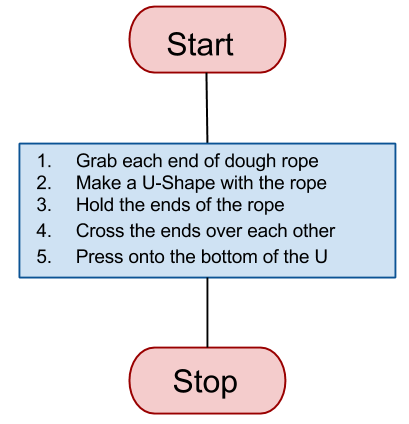
\includegraphics[width=.75\textwidth]{one_pretzel}
	\end{figure}
\end{frame}
%
\begin{frame}[fragile]{1 Pretzel}
\begin{minted}{c++}
#include<iostream>
using namespace std;

int main(){
    cout<<"Grab each end of dough rope"<<endl;
    cout<<"Make a U-Shape with the rope"<<endl;
    cout<<"Hold the ends of the rope"<<endl;
    cout<<"Cross the ends over each other"<<endl;
    cout<<"Press onto the bottom of the U"<<endl;
    return 0;
}
\end{minted}
\end{frame}

\begin{frame}{2 Pretzels}
\begin{figure}
		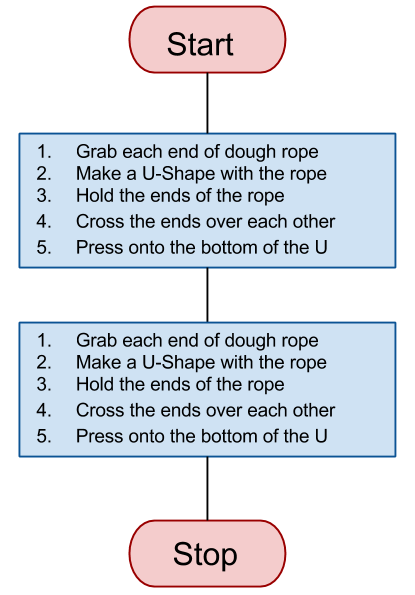
\includegraphics[width=.5\textwidth]{two_pretzels}
	\end{figure}
\end{frame}

\begin{frame}[fragile]{2 Pretzels}
\begin{minted}{c++}
#include<iostream>
using namespace std;

int main(){
    cout<<"Grab each end of dough rope"<<endl;
    cout<<"Make a U-Shape with the rope"<<endl;
    cout<<"Hold the ends of the rope"<<endl;
    cout<<"Cross the ends over each other"<<endl;
    cout<<"Press onto the bottom of the U"<<endl;
    cout<<"Grab each end of dough rope"<<endl;
    cout<<"Make a U-Shape with the rope"<<endl;
    cout<<"Hold the ends of the rope"<<endl;
    cout<<"Cross the ends over each other"<<endl;
    cout<<"Press onto the bottom of the U"<<endl;
    return 0;
}
\end{minted}
\end{frame}

\begin{frame}{N Pretzels}
\begin{figure}
		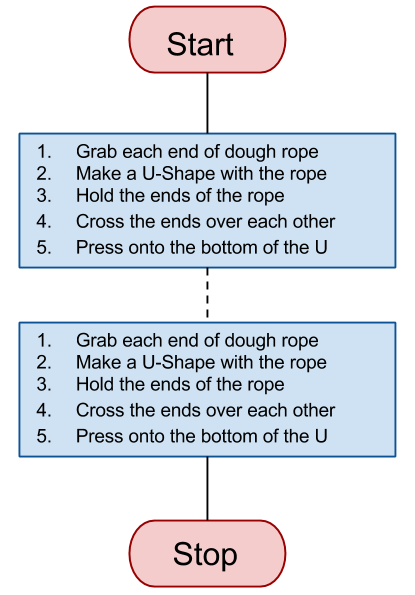
\includegraphics[width=.5\textwidth]{n_pretzels}
	\end{figure}
\end{frame}

\begin{frame}[fragile]{N Pretzels}
\begin{minted}{c++}
#include<iostream>
using namespace std;

int main(){
    cout<<"Grab each end of dough rope"<<endl;
    cout<<"Make a U-Shape with the rope"<<endl;
    cout<<"Hold the ends of the rope"<<endl;
    cout<<"Cross the ends over each other"<<endl;
    cout<<"Press onto the bottom of the U"<<endl;
    //copy and paste above N-2 times
    cout<<"Grab each end of dough rope"<<endl;
    cout<<"Make a U-Shape with the rope"<<endl;
    cout<<"Hold the ends of the rope"<<endl;
    cout<<"Cross the ends over each other"<<endl;
    cout<<"Press onto the bottom of the U"<<endl;
    return 0;
}
\end{minted}
\end{frame}

\begin{frame}{100 Pretzels}
\begin{figure}
		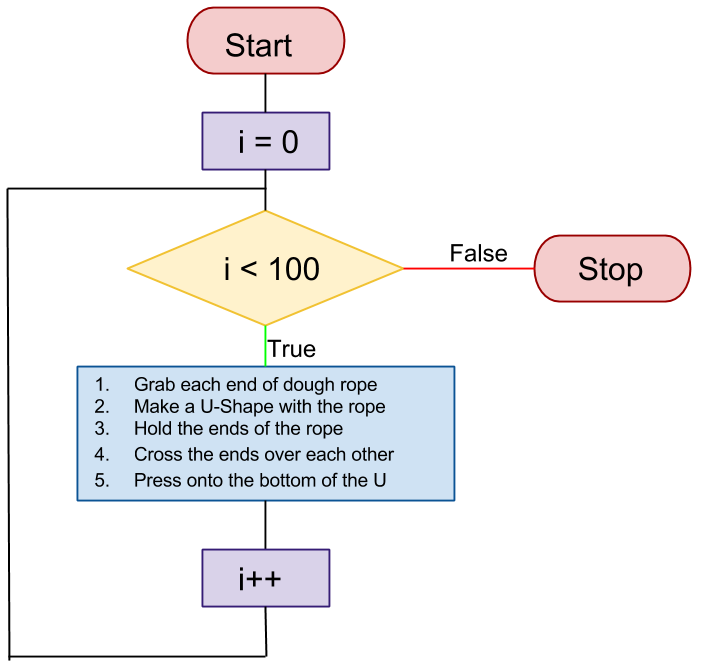
\includegraphics[width=.75\textwidth]{for_pretzels}
	\end{figure}
\end{frame}

\begin{frame}[fragile]{2 Pretzels}
\begin{minted}{c++}
#include<iostream>
using namespace std;

int main(){
    for(int i=0; i<100; i++){
        cout<<"Grab each end of dough rope"<<endl;
        cout<<"Make a U-Shape with the rope"<<endl;
        cout<<"Hold the ends of the rope"<<endl;
        cout<<"Cross the ends over each other"<<endl;
        cout<<"Press onto the bottom of the U"<<endl;
    }
    return 0;
}
\end{minted}
\end{frame}

\begin{frame}[fragile]{Number Line}
\begin{figure}
	\begin{minted}{c++}
         	    for(start; stop; step)
	\end{minted}
	\pause
	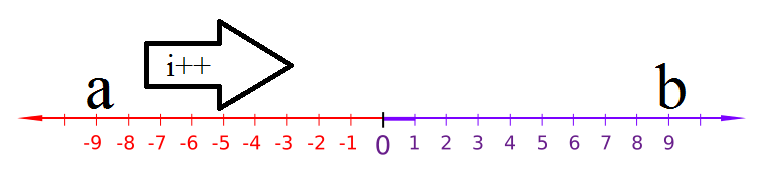
\includegraphics[width=1\textwidth]{nlpp}
	\begin{minted}{c++}
         	    for(int i=a; i<b; i++)
	\end{minted}
\end{figure}
\end{frame}


\begin{frame}[fragile]{Number Line}
\begin{figure}
	\begin{minted}{c++}
         	    for(int i=a; i<b; i++)
	\end{minted}
	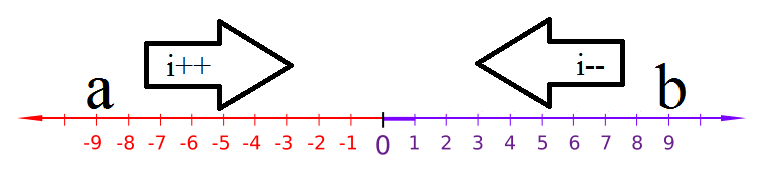
\includegraphics[width=1\textwidth]{nlmm}
	\begin{minted}{c++}
         	    for(int i=b; i>a; i--)
	\end{minted}
\end{figure}
\pause
\begin{center}
	\begin{itemize}
	\item Valid Steps: ++, --, +=C, -=C, /=C, *=C,
	\item Valid C:
		\begin{itemize} 
		\item any number
		\item function that evaluates to a number 
		\end{itemize}
	\end{itemize}
\end{center}

\end{frame}

\begin{frame}{Practice}
	\begin{enumerate}
		\item Write a program that prints out the numbers between 0 and 10
		\item Print out all the odd numbers between 0 and 10, inclusive
		\item Display the multples of 3 backward from 33 to 3, inclusive
	\end{enumerate}
\end{frame}

\begin{frame}{Common Loop Applications}
	\begin{block}{Summation}
		\begin{center}
		x = $\displaystyle \sum^{b}_{i=a} i \Leftrightarrow$ for(int i=a; i$<=$b; i++)\{x\textcolor{LimeGreen}{\textbf{+}}=i;\}
		\end{center}
	\end{block}
	\pause
	\begin{block}{Product}
		\begin{center}
		x = $\displaystyle \prod^{b}_{i=a} i \Leftrightarrow$ for(int i=a; i$<=$b; i++)\{x\textcolor{LimeGreen}{\textbf{*}}=i;\}
		\end{center}
	\end{block}
\end{frame}


\begin{frame}{Practice}
	\begin{enumerate}
		\item Write a program that prints out n!
		\item Write, run, and test a C++ program to find the value of $2^{n}$ by using a for loop, where n is an integer value the user enters at the keyboard. (Hint: Initialize result = 1. Accumulate result = 2 * result.
	\end{enumerate}
\end{frame}

\begin{frame}{Nesting Loops}
\begin{figure}
		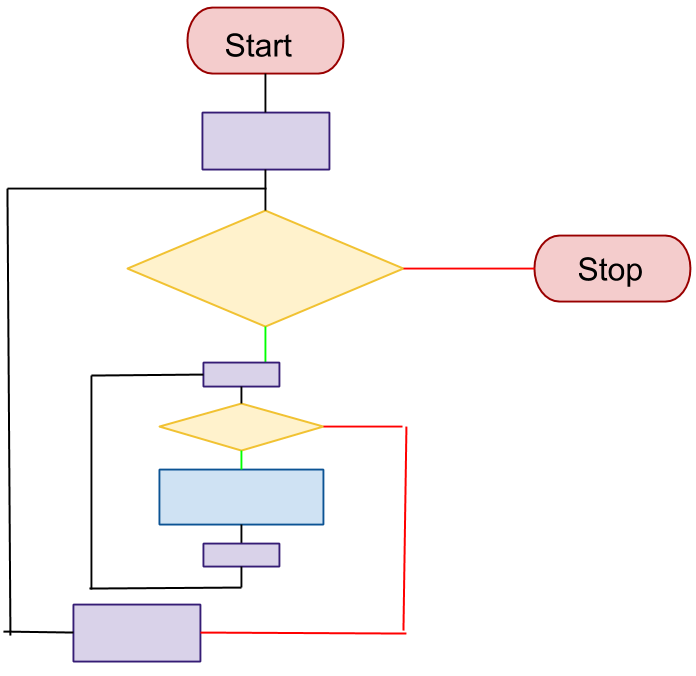
\includegraphics[width=.75\textwidth]{for_nests}
	\end{figure}
\end{frame}

\begin{frame}[fragile]{Nested Loops}
\begin{minted}{c++}
#include<iostream>
using namespace std;

int main(){
    for(start; stop; step){
        //body of outer for
        for{start; stop; step}{
            //inner for loop
        }
       //more code for outer loop
    }
return 0;
}
\end{minted}
\end{frame}

\begin{frame}{Practice}
	\begin{enumerate}
		\item Write a program to print out an n*n multiplication table
		\item Write a program that calculates and displays values for y when y = xz / (x - z):
			\begin{itemize}
				\item x ranging between 1 and 5 
				\item z ranging between 2 and 6
			\end{itemize}
	\end{enumerate}
\end{frame}

\end{document}

